\section{Introduction}
\label{sec:intro}

Recent years saw a rapid emergence of online dating as an acceptable means of meeting romantic interests.
While a somewhat taboo subject, and a source of some insecurity and hardship for many, dating sites allowed persons equitable access to the dating market regardless of their ability to meet people in their day-to-day lives.
For obvious reasons, online dating carries with it some social stigma and risks, and users prefer to remain anonymous until they explicitly elect to reveal their identity to select individuals.

In fact, privacy and the expectation of anonymity are key to the success of a dating site, as it establishes a relatively safe, on-demand means to access an otherwise risky dating scene.
Users entrust a cache of valuable personal information such as their identity, location, personal preferences, and a wealth of information about personal beliefs [TODO - cite OKC matching blog post].
While the dating sites may do everything in their power to correctly implement their privacy policy and protect the identities of their users, the users themselves must take care to ensure they do not compromise their privacy by revealing identifiable information in a public profile.

De-anonymizing the profiles featured on a dating site is valuable, as it would yield significant amounts of private personal information pertaining to specific individuals.
Some motivations for determining identities of individuals on a dating site may be relatively benign, such as academic or marketing research, a population study, or law enforcement.
There exist legitimate reasons for an individual attempting to ascertain the identity associated with a dating site profile.
Unfortunately, there also exist numerous sinister reasons to de-anonymize dating site profiles, such as stalking, blackmail, public embarrassment, or otherwise offensive or criminal behavior.

It stands to reason that users' interpretation of a dating site's privacy allows them to delegate some responsibility for maintaining anonymity to the site, enabling a safe environment to share private information.
The site is responsible for correctly implementing their privacy policy, and doing everything in their power to protect the users' identities and information.
Of course no measure is enough to prevent a user from compromising their own privacy by posting identifiable information in their public profile.
Users of dating sites must be educated to understand this in order to avoid being vulnerable to loss of privacy.
In this work, we illustrate that this is indeed a common problem by de-anonymizing a large set of users of a popular dating site.

\subsection{Plan of Attack}
\label{sec:intro_plan_of_attack}

\begin{figure}[hbtp]
  \center{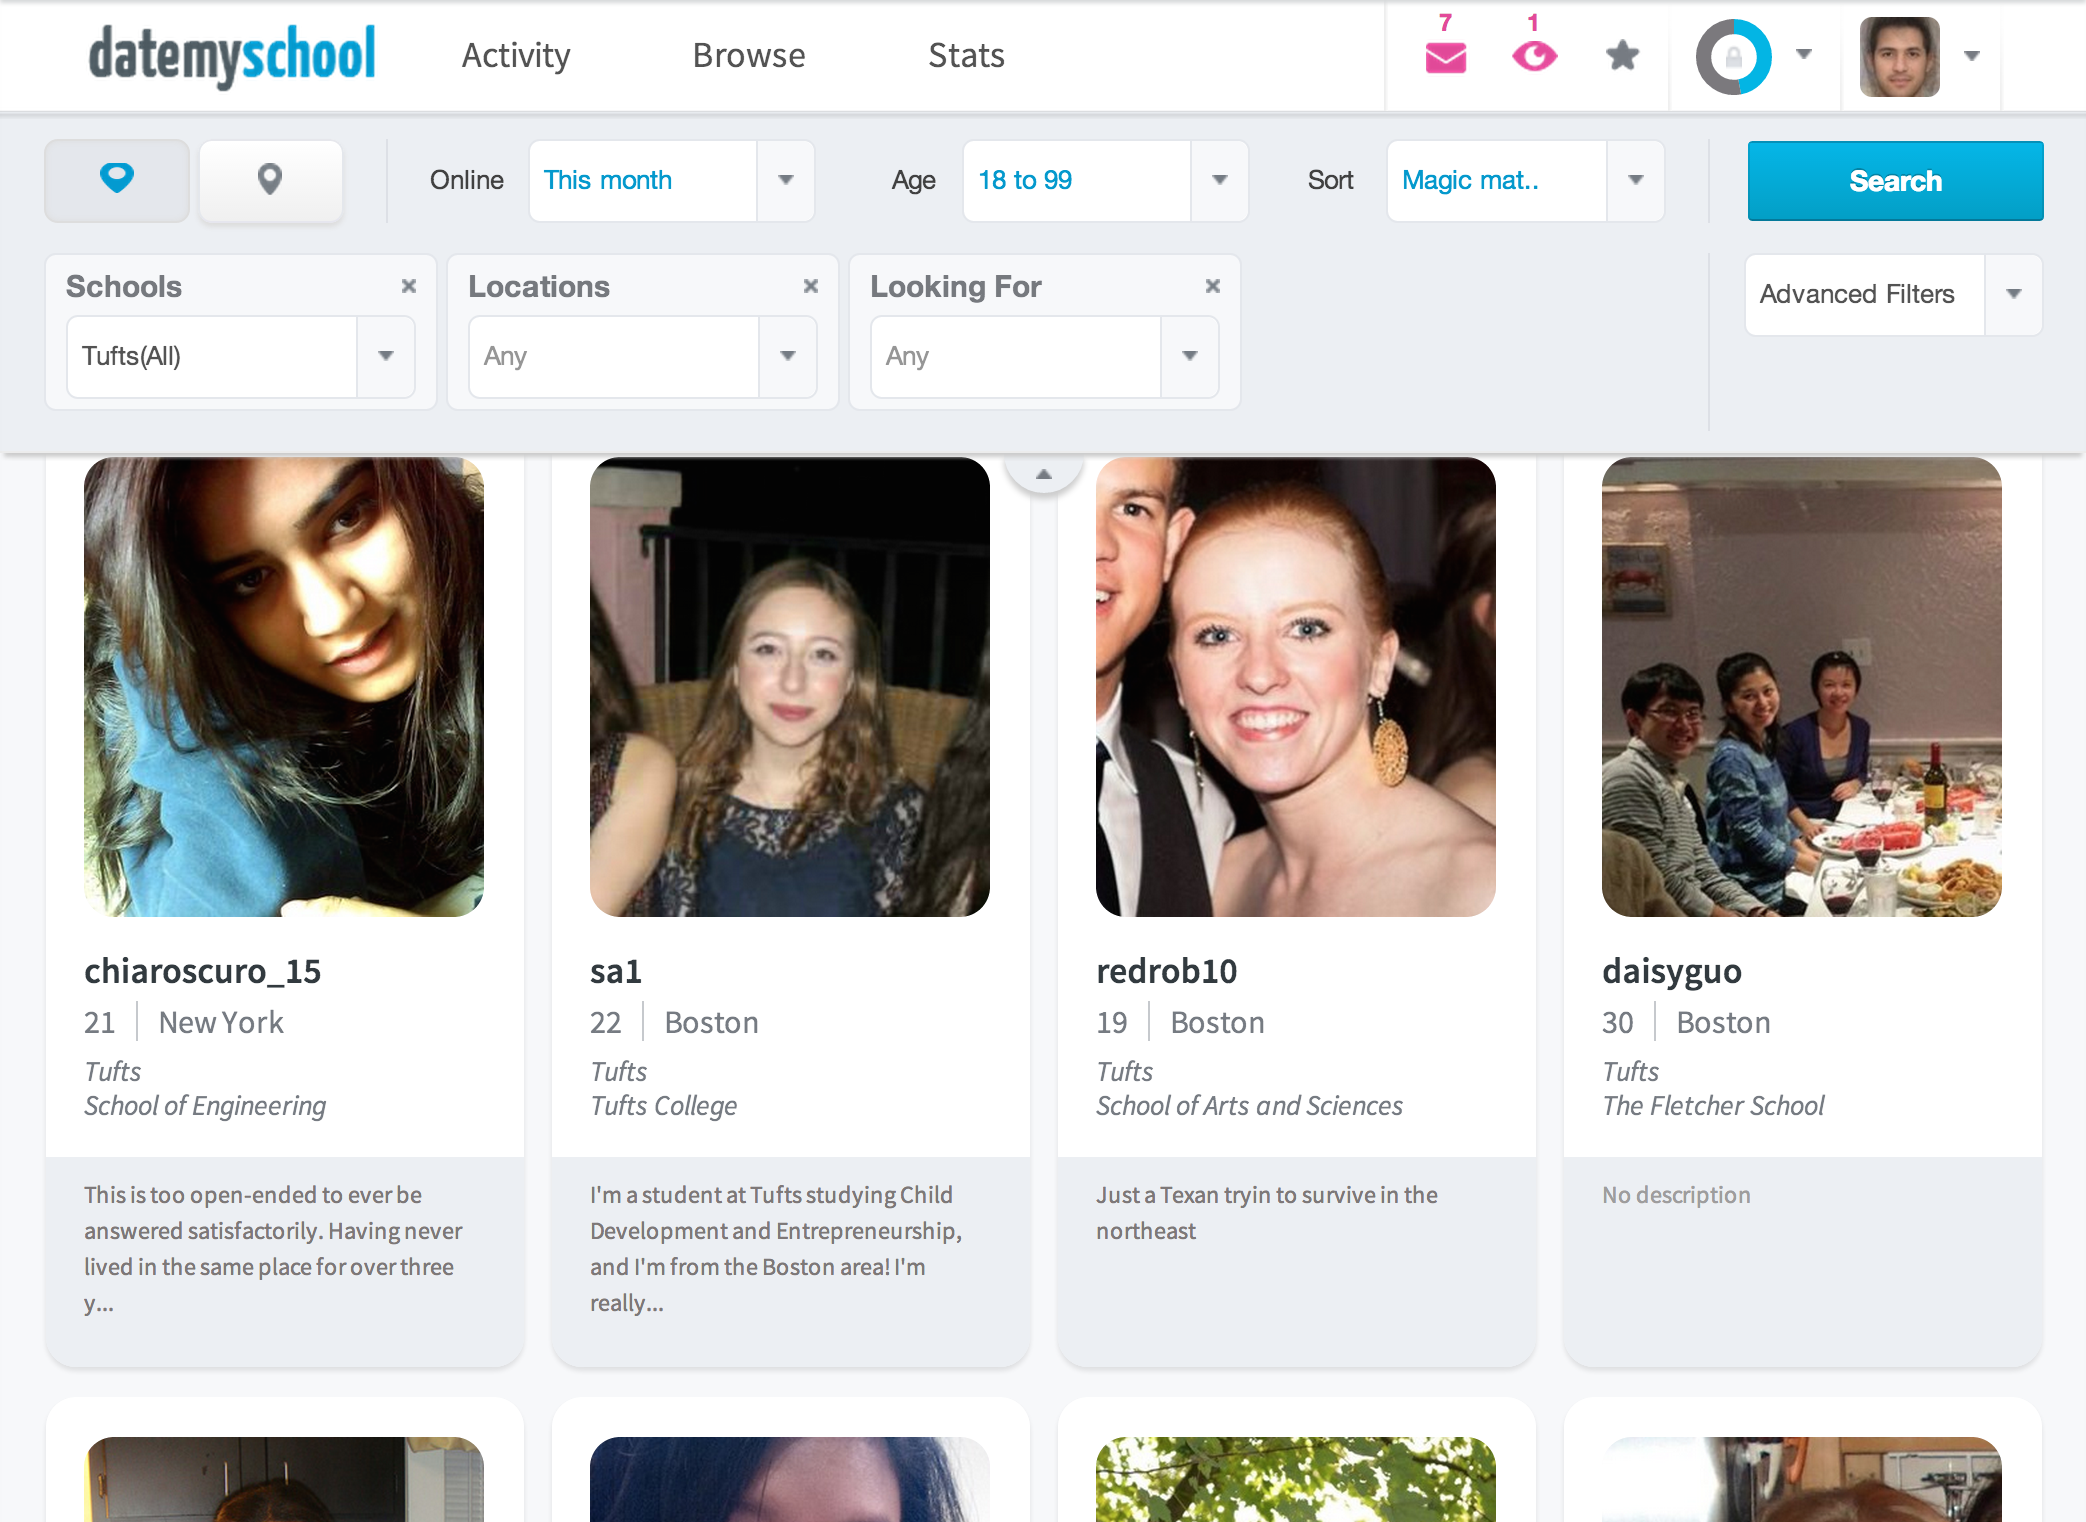
\includegraphics[width=85mm]{figures/dms_search.png}}
  \caption{
    A DateMySchool search for all the female Tufts students.
  }
  \label{fig:fb}
\end{figure}

\begin{figure}[hbtp]
  \center{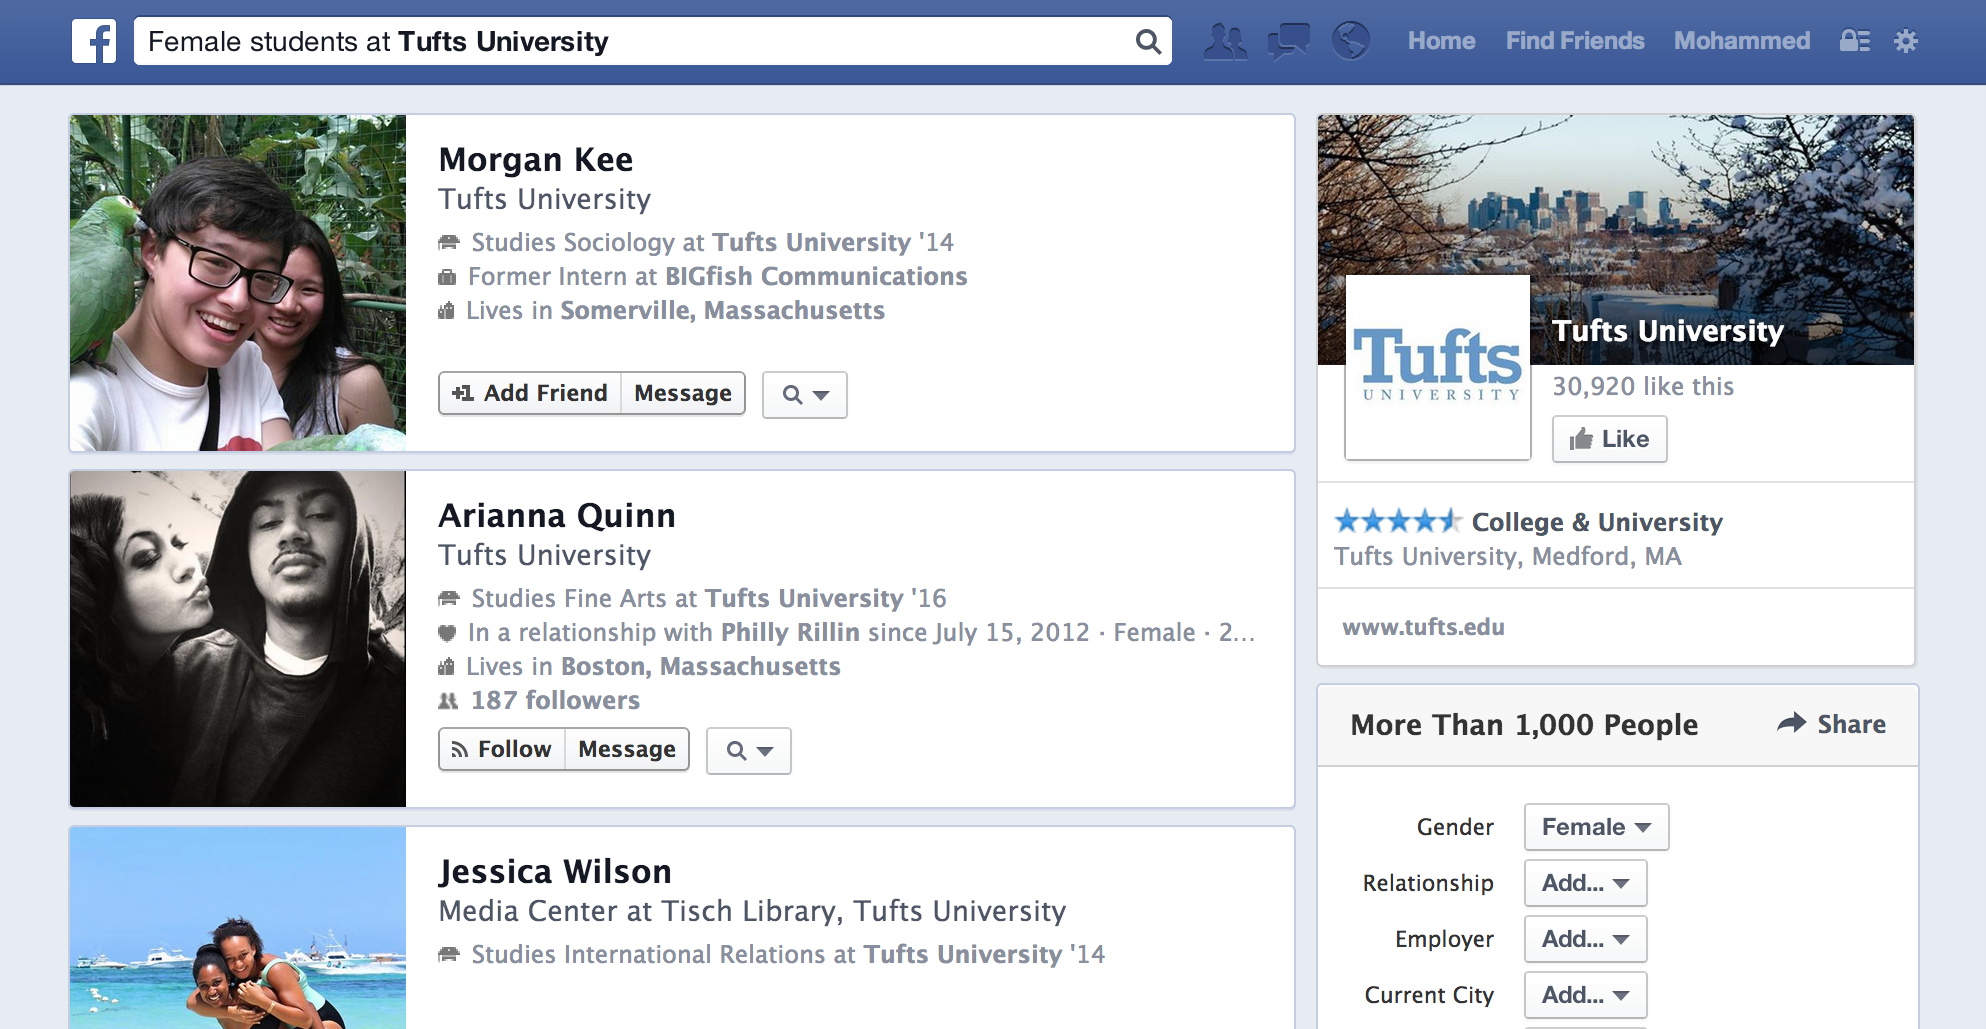
\includegraphics[width=85mm]{figures/fb_search.png}}
  \caption{
    A Facebook search for all the female Tufts students. The results are
    matched against the DateMySchool results for female students.
  }
  \label{fig:fb}
\end{figure}

% TODO: Tufts?
We enumerate a large set of (semi)-public but anonymous profiles featured on a the DMS(DateMySchool\cite{dms2014}) site by creating a fictitious account with the dating service and searching for users from Tufts university.
This site is popular with college students, as it groups users by school, thereby allowing users to explore the dating market within their academic institution, or with nearby academic institutions, supposedly reducing risk and improving match quality.
We also create a fictitious Facebook\cite{fb2014} account, and use it to extract a large body of non-anonymous profiles associated with the same university.
Facebook is very popular for its vast user base.
%TODO: does DMS actually require a linked FB account? -- nope, created the facebook way after the DMS account
%In fact, DMS requires a linked Facebook account to sign up, meaning we can expect with a high degree of confidence that each anonymous DMS profile has a non-anonymous Facebook profile.
We then use data set aggregation to correlate the anonymous dating site profiles to non-anonymous Facebook profiles using profile photographs of users as a common feature.
We conjecture that many users will reuse identical photographs on both sites, as they are motivated to select the photos that portray them in the best light.
Since most people have a relatively small set of recent photographs they consider flattering, it wouls stand to reason that their recent ``good'' photograph used to create a dating site profile would also be featured on Facebook.
Indeed, we found this to be the case with at least TODO\% of the accounts we attempted to de-anonymize.
